%%%%%%%%%%%%%%%%%%%%%%%%%%%%%%%%%%%%%%%%%%%%%%%%%%%%%%%%%%%%%%%%%%%
\section{Introduction}\label{sec:methodo_intro}

        La construction d'une plateforme de calcul \gls{exascale} nous oblige à relever de nombreux défis, présentés dans la \autoref{sec:challenges}. Nous avons vu que les pressions énergétiques et économiques obligeaient l'industrie à repenser les architectures et les technologies utilisées pour l'élaboration des plateformes de calcul haute performance. Dans la \autoref{sec:oppo}, nous avons listé les principales opportunités technologiques permettant de relever ces défis, parmis lesquelles:
        \begin{itemize} 
            \item le développement de technologies innovantes permettant l'élaboration d'architectures (voir \autoref{sec:new_soc});
            \item le développement du protocole universel \verb|Gen-Z| (voir \autoref{sec:gen_z}).
        \end{itemize}
        Ces deux opportunités vont permettre d'augmenter le niveau d'hétérogénéité des accélérateurs utilisés dans les supercalculateurs. Dans la \autoref{sec:edl_hpc_hetero}, nous avons expliqué pourquoi l'utilisation d'architectures hétérogènes dans un même calculateur était indispensable pour répondre aux défis que représente l'élaboration de plateformes \glspl{exascale}. Depuis 2010, l'utilisation d'un accélérateur pour assister le travail des processeurs est de plus en plus répandue. Bien que cette évolution semble se confirmer, il est important de s'intéresser à la nature des accélérateurs utilisés en 2018\footnote{Données calculées à partir du classement du Top500 de novembre 2018 - \url{https://www.top500.org/lists/2018/11/}}:
        \begin{itemize}
            \item 96\% des processeurs ont une architecture x86
            \item 91\% des processeurs sont produits par le constructeur Intel.
            \item 92\% des accélérateurs utilisés sont des GPU produits par Nvidia. 
        \end{itemize}
        Ainsi, bien que le nombre de supercalculateur utilisant un accélérateur ait évolué ces dernières années (28\% d'entre-eux en 2018), il est intéressant de remarquer que ces plateformes sont très similaires: un processeur x86 (Intel) associé à un ou plusieurs GPU (Nvidia). La forte évolution du nombre de GPU constatée ces dernières années et la prédominance de l'utilisation des \gls{GPU} peut en partie être expliquée par leur efficacité pour exécuter les applications d'intelligence artificielle. Cependant, si leur exécution peut être réalisée par un seul type d'accélérateur, la majorité des applications de HPC sont composées de plusieurs \glspl{kernel} pouvant avoir des besoins très différents. Pour que ces applications puissent aussi profiter de l'hétérogénéité, les plateformes doivent posséder différents types d'accélérateurs pour y exécuter les noyaux de calcul d'une application.
        %Cependant, une particularité des applications d'apprentissage par machine est leur profil uniforme. 
        
        %GenZ        
        Cette vision que nous présentons va être facilité par le développement du protocole universel \verb|Gen-Z|\footnote{Gen-Z Introduction and Executive Summary - \url{https://genzconsortium.org/wp-content/uploads/2018/05/Gen-Z-Overview-V1.pdf}} (voir \autoref{sec:gen_z}). Grâce à \verb|Gen-Z| différents accélérateurs pourront facilement collaborer pour l'exécution optimale de ces applications. Avec le développement de \verb=Gen-Z=, le déplacement de données entre accélérateurs sera facilité et la difficulté d'agrégation de différents matériels sera réduite. Nous prédisons que ce protocole, présenté dans la \autoref{sec:gen_z}, va révolutionner le monde de l'informatique comme peu de technologies auparavant. Entre tous les bénéfices apportés par ce protocole, la faculté de faciliter l'hétérogénéité dans les supercalculateurs est sans doute la plus importante. 

\subsection{Contributions}
%%%%%%%%%%%%%%%%%%%%%%%%%%%%%%%%%%%%%%%%%%%%%%%

       Les gains de performance ne viendront pas seulement de l'utilisation d'accélérateurs puissants, mais de leur diversité et de la capacité des programmeurs à bien les utiliser. Malheureusement, en l'absence de méthodes d'analyse de la performance des codes, ces architectures innovantes sont potentiellement condamnées puisque peu d'experts savent les valoriser. Ces nouvelles technologies, très différentes de celles utilisées aujourd'hui (processeur x86, GPU, DRAM), doivent être caractérisées pour prédire le gain de performance atteignable par les applications. 
          
          
        Pour pouvoir profiter de ces technologies et les utiliser de façon optimale, nous avons présenté dans le chapitre précédent une suite de logiciels de caractérisation et d'analyse de performance:
        \begin{enumerate}
            \item \texttt{DML\_MEM}: un \gls{benchmark} mémoire permettant de caractériser la hiérarchie mémoire lors de l'exécution d'applications utilisant des accès mémoires par sauts (\gls{stride});
            
            \item \texttt{Kernel Generator}: un générateur de benchmarks permettant de caractériser les unités de calcul arithmétique;
            
            \item \texttt{YAMB}: un outil permettant de réaliser le suivi de l'activité du bus mémoire;
            
            \item \texttt{Oprofile++}: un l'outil d'analyse permettant d'extraire et de caractériser les zones de codes responsables de la majorité du temps d'exécution de l'application. 
        \end{enumerate}

        Dans ce chapitre, nous présentons une méthodologie en 5 étapes qui permet aux utilisateurs de modéliser les performances de leur code, de les projeter sur de nouvelles architectures et de les optimiser (voir \autoref{pic:methodologie_step_2}). L'objectif de ce chapitre est de présenter une méthodologie adaptée, permettant d'utiliser efficacement les outils développés durant ce travail de thèse afin de réaliser la caractérisation des architectures ainsi que le portage des applications sur ces nouveaux accélérateurs.
        
        
        \begin{figure}[h!]
        \center
        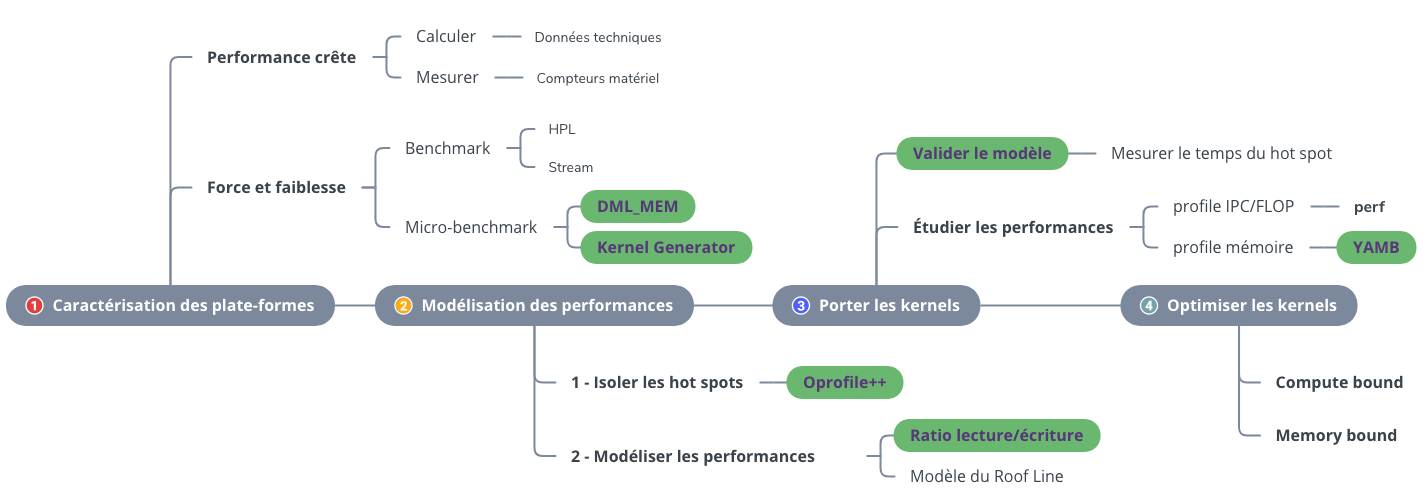
\includegraphics[width=17cm]{images/methodologie_step.png}
        \caption{\label{pic:methodologie_step_2} Méthodologie en 5 étapes pour caractériser et optimiser une application sur une nouvelle architecture.}
        \end{figure}
    
    
    \paragraph{Délimitation de l'analyse}
    %%%%%%%%%%%%%%%%%%%%%%%%%%%%%%%%%%%%%%%%%%%%%%%

        L'analyse et l'optimisation des performances d'une application peuvent être réalisées à plusieurs niveaux:  à l'échelle d'une grappe de serveurs, du processeur, d'un coeur, etc. Pour que le travail soit réalisable durant la thèse, nous avons délimité un certain cadre pour appliquer notre méthodologie (voir \autoref{pic_analyse}). Le premier cadre consiste à analyser les applications qui sont exécutées sur une plateforme homogène. C'est à dire que l'application est exécutée sur plusieurs serveurs avec la même configuration (matérielle et logicielle). Lorsque la programmation à mémoire distribuée a bien été réalisée, l'exécution sur les différents serveurs devrait être similaire. Notre analyse de performance peut alors se poursuivre sur un seul serveur. Les problèmes de performance liés à l'exécution sur plusieurs serveurs ne sont pas abordés dans cette analyse mais peuvent l'être grâce à l'utilisation d'outils tels que \verb=Extrae= \cite{Rodriguez}, \verb=Paraver= \cite{Pillet1995}  ou \verb=Tau= \cite{Shende2006}. Notre approche s'intéresse aux applications HPC, dont la majorité de l'exécution est passée à exécuter des instructions de calcul. Les applications dont la performance est limitée par celle du système de stockage, du réseau ou du système d'exploitation ne sont pas la priorité de la méthodologie présentée. Cependant, avec une certaine expérience ces limitations peuvent être identifiées par nos outils. Les applications que nous ciblons dans notre analyse sont des codes dont la majorité du temps d'exécution se déroule seulement dans quelques pourcentages des lignes de codes. Nous appelons ces zones des points chauds, \gls{hotspot} ou encore \glspl{kernel}. Une application possédant des hot spots est le gage d'un potentiel d'amélioration des performances. Notre approche s'intéresse particulièrement aux applications dont la performance est limitée par la performance du système mémoire (\gls{memorybound}) ou celle des unités de calcul (\gls{computebound}).
        
         \begin{figure}[h!]
            \center
            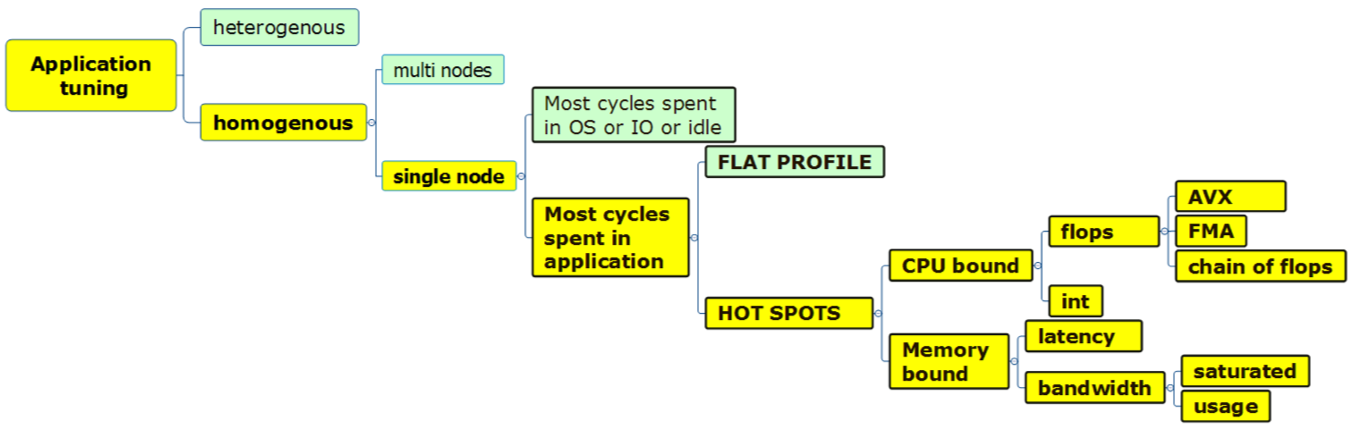
\includegraphics[width=16cm]{images/analyse.png}
            \caption{\label{pic_analyse} Délimitation de l'analyse proposée.}
        \end{figure}
        
     
        
        
\subsection{Organisation du chapitre}
%%%%%%%%%%%%%%%%%%%%%%%%%%%%%%%%%%%%%%%%%%%%%%%



    Ce chapitre présente les cinq étapes de la méthodologie et suit la structure suivante:
    \begin{itemize}
        \item La \autoref{sec:methodo_step1} présente la première étape qui consiste à se tenir au courant de toutes les nouveautés technologiques ayant un potentiel pour être utilisées dans les centres de calcul. Nous discutons des caractéristiques clefs qu'il est nécessaire de quantifier pour estimer le potentiel de chaque architecture.
        \item La \autoref{sec:methodo_step2} discute des méthodes pour calculer ou mesurer la performance d'une architecture. Nous montrons comment deux des outils présentés dans le chapitre précédent peuvent être utilisés pour cela.
        \item La \autoref{sec:methodo_step3} s'intéresse aux applications et notamment à la modélisation de leur performance. Pour ce faire, nous présentons différents outils permettant d'isoler les \glspl{hotspot} d'une application ainsi qu'un modèle de performance basé sur la performance du système mémoire.
        \item La \autoref{sec:methodo_step4} discute ensuite des principaux facteurs à étudier pour réaliser le choix des architectures à utiliser pour l'élaboration d'une nouvelle plateforme de calcul. 
        \item La \autoref{sec:methodo_step5} s'intéresse enfin au portage du code sur les plateformes sélectionnées précédemment. Nous y présentons une suite d'étapes à suivre pour valider la bonne performance des noyaux et, dans le cas contraire, les étapes à suivre pour optimiser leur performance.
    \end{itemize}
    
    Pour illustrer les différentes étapes, nous appliquons la méthodologie à l'étude des performances de la fonction \textit{triadd} (voir \autoref{lst:triadd}) du benchmark \verb|STREAM| \cite{McCalpin1995} sur un processeur Intel\textit{ Xeon Gold 6148} possédant 20 coeurs. Les matrices utilisées mesurent chacune 19.6 GB.\\
    
    \textbf{TODO check l'espace ici}
        
\begin{lstlisting}[language=c,caption={Fonction \textit{triad} extraite du benchmark \texttt{STREAM} \cite{McCalpin1995}.},label={lst:triadd}, 
  basicstyle=\footnotesize, frame=tb,
  xleftmargin=.065\textwidth, xrightmargin=.065\textwidth]
for (j=0; j < STREAM_ARRAY_SIZE; j++)
    A[j] = B[j] + scalar * C[j];
\end{lstlisting}






     
            
            %On peut en imaginer certains adaptés à la lecture et à la décompression du jeu de données. Une fois réalisés, des accélérateurs spécialisés dans le calcul demandé pourront être utilisés (ASIC, FGPA ou DSP). Enfin pour la visualisation des données, des GPU seront alors nécessaires. 


%Pour pouvoir profiter de l'hétérogénéité des accélérateurs, un travail préalable est nécessaire. Le premier est de caractériser ces plateformes, pour déterminer leurs forces, leurs faiblesses et leur efficacité pour un type d'application. Un second travail consiste à étudier l'application et à déterminer les besoins des noyaux de calculs la composant. La complexité de la microarchitecture peut lourdement impacter la performance d'une partie de l'application. Ainsi, notre démarche s'adresse aux programmeurs ayant de solides connaissances des microarchitectures. Les principales connaissances qui ont été requises pour développer cette méthodologie sont regroupées dans l'\aref{annexe:CHAPITRE_ARCHITECTURE}.
        
        %L'accès à des plateformes \glspl{exascale} et à ces nouvelles architectures va aussi ouvrir de nouveaux marchés, aujourd'hui à inaccessibles cause de plusieurs contraintes: le prix, la bande passante nécessaire, la sécurité ou encore la consommation électrique. 
